\item \points{30} {\bf Neural Networks: MNIST image classification}

In this problem, you will implement a simple neural network
to classify grayscale images of handwritten digits (0 - 9) from
the MNIST dataset. The dataset contains 60,000 training images and
10,000 testing images of handwritten digits, 0 - 9. Each image is
28$\times$28 pixels in size, and is generally represented as a flat
vector of 784 numbers. It also includes labels for each example, a number
indicating the actual digit (0 - 9) handwritten in that image. A sample of
a few such images are shown below.

\begin{center}
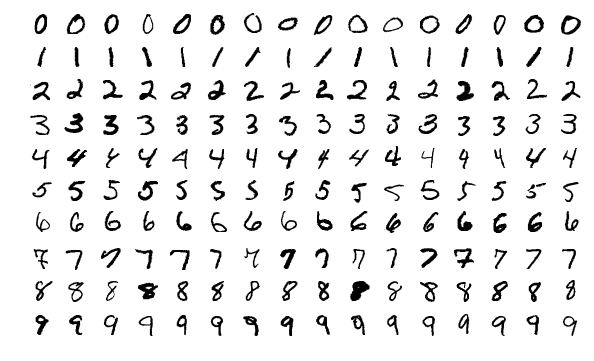
\includegraphics[scale=0.5]{mnist/mnist_plot}
\end{center}


The data and starter code for this problem can be found in

\begin{itemize}
\item \texttt{src/mnist/nn.py}
\item \texttt{src/mnist/images\_train.csv}
\item \texttt{src/mnist/labels\_train.csv}
\item \texttt{src/mnist/images\_test.csv}
\item \texttt{src/mnist/labels\_test.csv}
\end{itemize}

The starter code splits the set
of 60,000 training images and labels into a set of 50,000 examples as
the training set, and 10,000 examples for dev set.

To start, you will implement a neural network with a single hidden layer
and cross entropy loss, and train it with the provided data set. Use the
sigmoid function as activation for the hidden layer, and softmax function
for the output layer. Recall that for a single example $(x, y)$, the cross
entropy loss is:
$$CE(y, \hat{y}) = - \sum_{k=1}^K y_k \log \hat{y_k},$$
where $\hat{y} \in \mathbb{R}^{K}$ is the vector of softmax outputs
from the model for the training example $x$,
and $y \in \mathbb{R}^{K}$ is the ground-truth vector for the training example
$x$ such that $y = [0,...,0,1,0,...,0]^\top$ contains a single 1 at the
position of the correct class (also called a ``one-hot'' representation).

For clarity, we provide the forward propagation equations below for the neural network with a single hidden layer. We have labeled data $(x^{(i)}, y^{(i)})_{i=1}^n$, where $x^{(i)} \in \mathbb{R}^d$, and $y^{(i)} \in \mathbb{R}^K$ is a one-hot vector as described above. Let $h$ be the number of hidden units in the neural network, so that weight matrices $W^{[1]} \in \mathbb{R}^{d \times h}$ and $W^{[2]} \in \mathbb{R}^{h \times K}$. We also have biases $b^{[1]} \in \mathbb{R}^h$ and $b^{[2]} \in \mathbb{R}^K$. The forward propagation equations for a single input $x^{(i)}$ then are:

\begin{align*}
  a^{(i)} &= \sigma \left( {W^{[1]}}^\top x^{(i)}  + b^{[1]} \right)  \in \mathbb{R}^h \\
  z^{(i) }&= {W^{[2]}}^\top a^{(i)} + b^{[2]} \in \mathbb{R}^K \\
  \hat{y}^{(i)} &=  \mathrm{softmax}(z^{(i)}) \in \mathbb{R}^K
\end{align*}
where $\sigma$ is the sigmoid function. 

For $\nexp$ training examples, we average the cross entropy loss over the $\nexp$ examples.
  \begin{equation*}
  J(W^{[1]},W^{[2]},b^{[1]},b^{[2]}) = \frac{1}{\nexp}\sum_{i=1}^\nexp CE(y^{(i)}, \hat{y}^{(i)}) = - \frac{1}{\nexp}\sum_{i=1}^\nexp \sum_{k=1}^K y_k^{(i)} \log \hat{y}_k^{(i)}.
  \end{equation*}
The starter code already converts labels into one hot representations for you.

Instead of batch gradient descent or stochastic gradient descent, the common practice
is to use mini-batch gradient descent for deep learning tasks. In this case, the
cost function is defined as follows:

  \begin{equation*}
  J_{MB} = \frac{1}{B}\sum_{i=1}^{B}CE(y^{(i)}, \hat{y}^{(i)})
  \end{equation*}
where $B$ is the batch size, i.e. the number of training example in each mini-batch. 

\begin{enumerate}
  \item \points{5} 

%For a single input example $x^{(i)}$ with one-hot label vector $y^{(i)}$, show that $$\nabla_{z^{(i)}} \mathrm{CE}(y^{(i)}, \hat{y}^{(i)}) = \nabla_{z^{(i)}} \mathrm{CE}(y^{(i)}, \mathrm{softmax}(z^{(i)}) ) = \hat{y}^{(i)} - y^{(i)} \in \mathbb{R}^K$$
For a single input example $x^{(i)}$ with one-hot label vector $y^{(i)}$, show that $$\nabla_{z^{(i)}} \mathrm{CE}(y^{(i)}, \hat{y}^{(i)}) = \hat{y}^{(i)} - y^{(i)} \in \mathbb{R}^K$$

where $\zsi \in \mathbb{R}^K$ is the input to the softmax function, i.e. $$\hat{y}^{(i)} = \mathrm{softmax}(\zsi)$$

(Note: in deep learning, $\zsi$ is sometimes referred to as the "logits".)

\textbf{Hint:} To simplify your answer, it might be convenient to denote the true label of $x^{(i)}$ as $l \in \{1,\dots,K\}$. Hence $l$ is the index such that that $y^{(i)} = [0,...,0,1,0,...,0]^\top$ contains a single 1 at the $l$-th position. You may also wish to compute $\displaystyle \frac{\partial \mathrm{CE}(y^{(i)}, \hat{y}^{(i)})}{\partial z^{(i)}_j}$ for $j\neq l$ and $j=l$ separately.


\ifnum\solutions=1 {
  \begin{answer}

First, let's expand the expression $\mathrm{CE}(y^{(i)}, \hat{y}^{(i)})$.
  \begin{align*}
\mathrm{CE}(y^{(i)},\hat{y}^{(i)}) = & - \sum_{k=1}^K y^{(i)}_k \log \hat{y}^{(i)}_k =  - y^{(i)}_l \log \hat{y}^{(i)}_l = - \log \hat{y}^{(i)}_l \\
& =  - \log (\mathrm{softmax}(z^{(i)}) _l)  \\
& =  - \log (\mathrm{softmax}(z^{(i)}_l))  \\
& =  - \log \left[ \frac{\exp(z^{(i)}_l)}{\sum_{k=1}^K \exp(z_k^{(i)})} \right]  \\
& =  - z^{(i)}_l + \log \sum_{k=1}^K \exp(z^{(i)}_k)
  \end{align*}

  To determine the gradient, first let's consider $\displaystyle \frac{\partial \mathrm{CE}(y^{(i)},\hat{y}^{(i)}) }{ \partial z^{(i)}_l}$:
  \begin{align*}
  \frac{\partial \mathrm{CE}(y^{(i)},\hat{y}^{(i)}) }{ \partial z^{(i)}_l} &=  \frac{\partial  }{ \partial z^{(i)}_l}(-z^{(i)}_l + \log (\sum_{k=1}^K \exp(z^{(i)}_k))) = -1 + \frac{\exp(z^{(i)}_l)}{\sum_{k=1}^K \exp(z^{(i)}_k)} \\
  &= -1 + \mathrm{softmax}(z^{(i)})_l \\
  &= -y^{(i)}_l + \hat{y}^{(i)}_l.
  \end{align*}

  Now let's consider $\displaystyle \frac{\partial \mathrm{CE}(y^{(i)},\hat{y}^{(i)}) }{ \partial z^{[2]}_j}$ for $j \neq l$:
  \begin{align*}
  \frac{\partial \mathrm{CE}(y^{(i)},\hat{y}^{(i)}) }{ \partial z^{(i)}_j} &=  \frac{\partial  }{ \partial z^{(i)}_j}(- z^{(i)}_l + \log (\sum_{k=1}^K \exp(z^{(i)}_k))) = \frac{\exp(z^{(i)}_j)}{\sum_{k=1}^K \exp(z^{(i)}_k)} \\
  &= \mathrm{softmax}(z^{(i)})_j \\
  &= -y^{(i)}_j + \hat{y}^{(i)}_j
  \end{align*}

  Combining the two cases, we have $ \nabla_{z^{(i)}} \mathrm{CE}(y^{(i)}, \hat{y}^{(i)}) = \hat{y}^{(i)} - y^{(i)} $ as desired.

\end{answer}
   
  

} \fi

  \item \points{15} 

Implement both forward-propagation and back-propagation for the above loss function $J_{MB} = \frac{1}{B}\sum_{i=1}^{B}CE(y^{(i)}, \hat{y}^{(i)})$.
Initialize the weights of the network by sampling values from a standard normal
distribution. Initialize the bias/intercept term to 0.
Set the number of hidden units to be 300, and learning rate to be 5. Set $B = 1,000$
(mini batch size). This means that we train with 1,000 examples in each iteration.
Therefore, for each epoch, we need 50 iterations to cover the entire training data.
The images are pre-shuffled. So you don't need to randomly sample the data, and can
just create mini-batches sequentially.


Train the model with mini-batch gradient descent
as described above. Run the training for 30 epochs. At the end of each epoch, calculate
the value of loss function averaged over the entire training set, and plot it
(y-axis) against the number of epochs (x-axis). In the same image, plot the value
of the loss function averaged over the dev set, and plot it against the number of epochs.

Similarly, in a new image, plot the accuracy (on y-axis) over the training set,
measured as the fraction of correctly classified examples, versus the number of epochs
(x-axis). In the same image, also plot the accuracy over the dev set versus number of epochs.

\textbf{Submit the two plots (one for loss vs epoch, another for accuracy vs epoch) in your writeup.}

Also, at the end of 30 epochs, save the learnt parameters (i.e all the weights and biases)
into a file, so that next time you can directly initialize the parameters with
these values from the file, rather than re-training all over. You do NOT need to
submit these parameters.


\textbf{Hint:} Be sure to vectorize your code as much as possible! Training can be
very slow otherwise.


\ifnum\solutions=1 {
  \begin{answer}
Unregularized loss curves

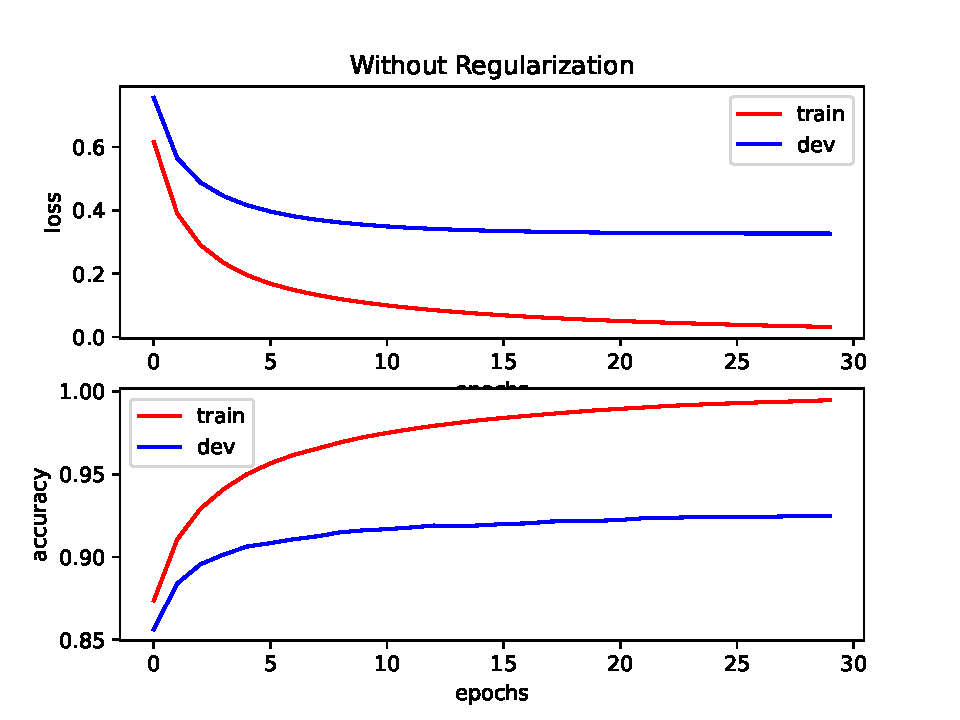
\includegraphics[scale=0.75]{../src/mnist/baseline}

\textbf{Note: \\ Derivation of the gradients for mini-batch gradient descent:}

First, the dimensions of the training data are $X \in \mathbb{R}^{B \times d}$, $y  \in \mathbb{R}^{B \times K}$, and the dimensions of the parameters are $W^{[1]}  \in \mathbb{R}^{d \times h}$, $b^{[1]}  \in \mathbb{R}^{h}$, $W^{[2]}  \in \mathbb{R}^{h \times K}$, $b^{[2]}  \in \mathbb{R}^{K}$.

The forward propagation equations in a vectorized form are:
\begin{align*}
    z^{[1]} &= X W^{[1]} + \tilde{b}^{[1]} &&\in \mathbb{R}^{B \times h}\\
    a &= \sigma \left( z^{[1]} \right) &&\in \mathbb{R}^{B \times h}\\
    z &= a W^{[2]} + \tilde{b}^{[2]} &&\in \mathbb{R}^{B \times K}\\
    \hat{y} &= \text{softmax} \left( z \right) &&\in \mathbb{R}^{B \times K}
\end{align*}
Note that $\tilde{b}$ terms are the broadcasted version of $b$ terms.
For further detail, see the lecture note on Deep learning.

Then, the gradients of $J_{MB}$ with respect to each variable/parameter are:
\begin{align*}
    \nabla_{z} J_{MB} &= \frac{1}{B} \nabla_{z} \mathrm{CE}(y, \hat{y}) &&= \frac{1}{B} \left( \hat{y} - y \right) & &\in \mathbb{R}^{B \times K}\\
    \nabla_{W^{[2]}} J_{MB} &= \frac{1}{B} \nabla_{W^{[2]}} \mathrm{CE}(y, \hat{y}) &&= 
    \frac{1}{B} \underbrace{a^T}_{(h \times B)}  \cdot \underbrace{\left( \hat{y} - y \right)}_{(B \times K)} & &\in \mathbb{R}^{h \times K}\\
    \nabla_{b^{[2]}} J_{MB} &= \frac{1}{B} \nabla_{b^{[2]}} \mathrm{CE}(y, \hat{y}) &&= 
    \frac{1}{B} \underbrace{\vec{\mathbf{1}}}_{(B,)} \cdot \underbrace{\left( \hat{y} - y \right)}_{(B \times K)} & &\in \mathbb{R}^{K}\\
    \nabla_{a} J_{MB} &= \frac{1}{B} \nabla_{a} \mathrm{CE}(y, \hat{y}) &&= 
    \frac{1}{B} \underbrace{\left( \hat{y} - y \right)}_{(B \times K)} \cdot \underbrace{W^{[2]T}}_{(K \times h)} & &\in \mathbb{R}^{B \times h}\\
    \nabla_{z^{[1]}} J_{MB} &= \frac{1}{B} \nabla_{z^{[1]}} \mathrm{CE}(y, \hat{y}) &&= 
    \frac{1}{B} \underbrace{a \odot (1-a)}_{(B \times h)} \odot
    \underbrace{ \left[ \left( \hat{y} - y \right) \cdot W^{[2]T} \right]}_{(B \times h)}
    & &\in \mathbb{R}^{B \times h}\\
    \nabla_{W^{[1]}} J_{MB} &= \frac{1}{B} \nabla_{W^{[1]}} \mathrm{CE}(y, \hat{y}) &&= 
    \frac{1}{B} \underbrace{X^T}_{(d \times B)} \underbrace{ \left[ a \odot (1-a) \odot
    \left( \hat{y} - y \right) \cdot W^{[2]T} \right]}_{(B \times h)} & &\in \mathbb{R}^{d \times h}\\
    \nabla_{b^{[1]}} J_{MB} &= \frac{1}{B} \nabla_{b^{[1]}} \mathrm{CE}(y, \hat{y}) &&= 
    \frac{1}{B} \underbrace{\vec{\mathbf{1}}}_{(B,)} \cdot \underbrace{ \left[ a \odot (1-a) \odot
    \left( \hat{y} - y \right) \cdot W^{[2]T} \right]}_{(B \times h)} & &\in \mathbb{R}^{h}
\end{align*}

\end{answer}
   
  

} \fi

  \item \points{7} Now add a regularization term to your cross entropy loss.
The loss function will become \begin{equation*}
  J_{MB} = \left(\frac{1}{B}\sum_{i=1}^{B}CE(y^{(i)}, \hat{y}^{(i)})\right) + \lambda \left(||W^{[1]}||^2 + ||W^{[2]}||^2 \right)
  \end{equation*}

Be careful not to regularize the bias/intercept term.
Set $\lambda$ to be 0.0001. Implement the regularized version and plot the same
figures as part (a). Be careful NOT to include the regularization term to measure
the loss value for plotting (i.e., regularization should only be used for gradient calculation for
the purpose of training).

\textbf{Submit the two new plots obtained with regularized training (i.e loss (without regularization term) vs epoch, and accuracy vs epoch) in your writeup.}

\textbf{Compare the plots obtained from the regularized model with the plots obtained
from the non-regularized model, and summarize your observations in a couple of sentences.}

As in the previous part, save the learnt parameters (weights and biases) into a
different file so that we can initialize from them next time.



\ifnum\solutions=1 {
  \begin{answer}
Regularized loss curves

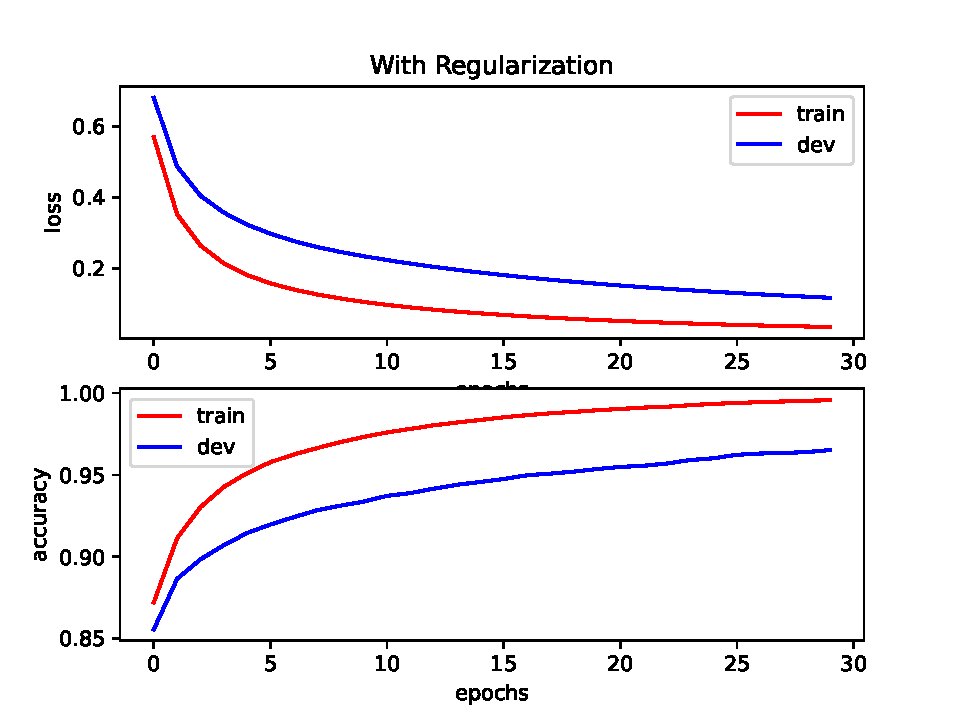
\includegraphics[scale=0.75]{../src/mnist/regularized}

The gap of accuracy between training set and dev set is smaller for regularize version.
Regularization helps avoid over-fitting!\\

\textbf{Note: \\ Derivation of the gradients for mini-batch gradient descent with regularization:}
The gradients of $J_{MB}$ with respect to the weight terms with the regularization term change to:

\begin{align*}
\nabla_{W^{[2]}} J_{MB} &=
\frac{1}{B} a^T  \cdot \left( \hat{y} - y \right) + 2 \lambda W^{[2]} & &\in \mathbb{R}^{h \times K}\\
\nabla_{W^{[1]}} J_{MB} &=
\frac{1}{B} X^T \left[ a \odot (1-a) \odot
\left( \hat{y} - y \right) \cdot W^{[2]T} \right]  + 2 \lambda W^{[1]} & &\in \mathbb{R}^{d \times h}
\end{align*}

The gradients with respect to the bias/intercept terms are not affected by regularization.
  
\end{answer}
   
  

} \fi


  \item \points{3}
All this while you should have stayed away from the test data completely. Now that
you have convinced yourself that the model is working as expected (i.e, the
observations you made in the previous part matches what you learnt in class
about regularization), it is finally time to measure the model performance on
the test set. Once we measure the test set performance, we report it (whatever
value it may be), and NOT go back and refine the model any further.

Initialize your model from the parameters saved in part (a) (i.e, the non-regularized
model), and evaluate the model performance on the test data. Repeat this using the
parameters saved in part (b) (i.e, the regularized model).

Report your test accuracy for both regularized model and non-regularized model.  
Briefly (in one sentence) explain why this outcome makes sense"
You should have accuracy close to 0.92870 without regularization, and 0.96760 with regularization.
Note: these accuracies assume you implement the code with the matrix dimensions as specified in
the comments, which is not the same way as specified in your code. Even if you do not precisely these
numbers, you should observe good accuracy and better test accuracy with regularization.


\ifnum\solutions=1 {
  \begin{answer}
It makes sense the regularized version does better on test set, since regularization is meant to help with avoiding overfitting to the train data.
\end{answer}
   
  

} \fi

 \end{enumerate}

